% $Header: /cvsroot/latex-beamer/latex-beamer/examples/beamerexample5.tex,v 1.22 2004/10/08 14:02:33 tantau Exp $

\documentclass[11pt]{beamer}

\usetheme{Darmstadt}

\usepackage{times}
\usefonttheme{structurebold}

%\usepackage[english]{babel}
\usepackage[portuges]{babel}
\usepackage{pgf,pgfarrows,pgfnodes,pgfautomata,pgfheaps}
\usepackage{amsmath,amssymb}
%\usepackage[latin8]{inputenc}
\usepackage[utf8]{inputenc}
\usepackage{graphicx}

\setbeamercovered{dynamic}

\newcommand{\Lang}[1]{\operatorname{\text{\textsc{#1}}}}

\newcommand{\Class}[1]{\operatorname{\mathchoice
  {\text{\sf \small #1}}
  {\text{\sf \small #1}}
  {\text{\sf #1}}
  {\text{\sf #1}}}}

\newcommand{\NumSAT}      {\text{\small\#SAT}}
\newcommand{\NumA}        {\#_{\!A}}

\newcommand{\barA}        {\,\bar{\!A}}

\newcommand{\Nat}{\mathbb{N}}
\newcommand{\Set}[1]{\{#1\}}

\pgfdeclaremask{tu}{beamer-tu-logo-mask}
\pgfdeclaremask{computer}{beamer-computer-mask}
\pgfdeclareimage[interpolate=true,mask=computer,height=2cm]{computerimage}{beamer-computer}
\pgfdeclareimage[interpolate=true,mask=computer,height=2cm]{computerworkingimage}{beamer-computerred}
\pgfdeclareimage[mask=tu,height=.5cm]{logo}{logounesp}

\logo{\pgfuseimage{logo}}

\title{Potenciais Unidimensionais}
\author{Ney Lemke}
\institute[IBB-UNESP]{%
    Mec\^anica Qu\^antica}
\date{2011}                                

\colorlet{redshaded}{red!25!bg}
\colorlet{shaded}{black!25!bg}
\colorlet{shadedshaded}{black!10!bg}
\colorlet{blackshaded}{black!40!bg}

\colorlet{darkred}{red!80!black}
\colorlet{darkblue}{blue!80!black}
\colorlet{darkgreen}{green!80!black}

\def\radius{0.96cm}
\def\innerradius{0.85cm}

\def\softness{0.4}
\definecolor{softred}{rgb}{1,\softness,\softness}
\definecolor{softgreen}{rgb}{\softness,1,\softness}
\definecolor{softblue}{rgb}{\softness,\softness,1}

\definecolor{softrg}{rgb}{1,1,\softness}
\definecolor{softrb}{rgb}{1,\softness,1}
\definecolor{softgb}{rgb}{\softness,1,1}

\newcommand{\Bandshaded}[2]{
  \color{shadedshaded}
  \pgfmoveto{\pgfxy(-0.5,0)}
  \pgflineto{\pgfxy(-0.6,0.1)}
  \pgflineto{\pgfxy(-0.4,0.2)}
  \pgflineto{\pgfxy(-0.6,0.3)}
  \pgflineto{\pgfxy(-0.4,0.4)}
  \pgflineto{\pgfxy(-0.5,0.5)}
  \pgflineto{\pgfxy(4,0.5)}
  \pgflineto{\pgfxy(4.1,0.4)}
  \pgflineto{\pgfxy(3.9,0.3)}
  \pgflineto{\pgfxy(4.1,0.2)}
  \pgflineto{\pgfxy(3.9,0.1)}
  \pgflineto{\pgfxy(4,0)}
  \pgfclosepath
  \pgffill

  \color{black}  
  \pgfputat{\pgfxy(0,0.7)}{\pgfbox[left,base]{#1}}
  \pgfputat{\pgfxy(0,-0.1)}{\pgfbox[left,top]{#2}}
}

\newcommand{\Band}[2]{
  \color{shaded}
  \pgfmoveto{\pgfxy(-0.5,0)}
  \pgflineto{\pgfxy(-0.6,0.1)}
  \pgflineto{\pgfxy(-0.4,0.2)}
  \pgflineto{\pgfxy(-0.6,0.3)}
  \pgflineto{\pgfxy(-0.4,0.4)}
  \pgflineto{\pgfxy(-0.5,0.5)}
  \pgflineto{\pgfxy(4,0.5)}
  \pgflineto{\pgfxy(4.1,0.4)}
  \pgflineto{\pgfxy(3.9,0.3)}
  \pgflineto{\pgfxy(4.1,0.2)}
  \pgflineto{\pgfxy(3.9,0.1)}
  \pgflineto{\pgfxy(4,0)}
  \pgfclosepath
  \pgffill

  \color{black}  
  \pgfputat{\pgfxy(0,0.7)}{\pgfbox[left,base]{#1}}
  \pgfputat{\pgfxy(0,-0.1)}{\pgfbox[left,top]{#2}}
}

\newcommand{\BaenderNormal}
{%
  \pgfsetlinewidth{0.4pt}
  \color{black}
  \pgfputat{\pgfxy(0,5)}{\Band{input tapes}{}}
  \pgfputat{\pgfxy(0.35,4.6)}{\pgfbox[center,base]{$\vdots$}}
  \pgfputat{\pgfxy(0,4)}{\Band{}{}}

  \pgfxyline(0,5)(0,5.5)
  \pgfxyline(1.2,5)(1.2,5.5)
  \pgfputat{\pgfxy(0.25,5.25)}{\pgfbox[left,center]{$w_1$}}

  \pgfxyline(0,4)(0,4.5)
  \pgfxyline(1.8,4)(1.8,4.5)        
  \pgfputat{\pgfxy(0.25,4.25)}{\pgfbox[left,center]{$w_n$}}
  \ignorespaces}

\newcommand{\BaenderZweiNormal}
{%
  \pgfsetlinewidth{0.4pt}
  \color{black}
  \pgfputat{\pgfxy(0,5)}{\Band{Zwei Eingabeb\~AƒÂƒ\~A‚¤nder}{}}
  \pgfputat{\pgfxy(0,4.25)}{\Band{}{}}

  \pgfxyline(0,5)(0,5.5)
  \pgfxyline(1.2,5)(1.2,5.5)
  \pgfputat{\pgfxy(0.25,5.25)}{\pgfbox[left,center]{$u$}}

  \pgfxyline(0,4.25)(0,4.75)
  \pgfxyline(1.8,4.25)(1.8,4.75)        
  \pgfputat{\pgfxy(0.25,4.5)}{\pgfbox[left,center]{$v$}}
  \ignorespaces}

\newcommand{\BaenderHell}
{%
  \pgfsetlinewidth{0.4pt}
  \color{black}
  \pgfputat{\pgfxy(0,5)}{\Bandshaded{input tapes}{}}
  \color{shaded}
  \pgfputat{\pgfxy(0.35,4.6)}{\pgfbox[center,base]{$\vdots$}}
  \pgfputat{\pgfxy(0,4)}{\Bandshaded{}{}}

  \color{blackshaded}
  \pgfxyline(0,5)(0,5.5)
  \pgfxyline(1.2,5)(1.2,5.5)
  \pgfputat{\pgfxy(0.25,5.25)}{\pgfbox[left,center]{$w_1$}}

  \pgfxyline(0,4)(0,4.5)
  \pgfxyline(1.8,4)(1.8,4.5)        
  \pgfputat{\pgfxy(0.25,4.25)}{\pgfbox[left,center]{$w_n$}}
  \ignorespaces}

\newcommand{\BaenderZweiHell}
{%
  \pgfsetlinewidth{0.4pt}
  \color{black}
  \pgfputat{\pgfxy(0,5)}{\Bandshaded{Zwei Eingabeb\~AƒÂƒ\~A‚¤nder}{}}%
  \color{blackshaded}
  \pgfputat{\pgfxy(0,4.25)}{\Bandshaded{}{}}
  \pgfputat{\pgfxy(0.25,4.5)}{\pgfbox[left,center]{$v$}}
  \pgfputat{\pgfxy(0.25,5.25)}{\pgfbox[left,center]{$u$}}%

  \pgfxyline(0,5)(0,5.5)
  \pgfxyline(1.2,5)(1.2,5.5)

  \pgfxyline(0,4.25)(0,4.75)
  \pgfxyline(1.8,4.25)(1.8,4.75)        
  \ignorespaces}

\newcommand{\Slot}[1]{%
  \begin{pgftranslate}{\pgfpoint{#1}{0pt}}%
    \pgfsetlinewidth{0.6pt}%
    \color{structure}%
    \pgfmoveto{\pgfxy(-0.1,5.5)}%
    \pgfbezier{\pgfxy(-0.1,5.55)}{\pgfxy(-0.05,5.6)}{\pgfxy(0,5.6)}%
    \pgfbezier{\pgfxy(0.05,5.6)}{\pgfxy(0.1,5.55)}{\pgfxy(0.1,5.5)}%
    \pgflineto{\pgfxy(0.1,4.0)}%
    \pgfbezier{\pgfxy(0.1,3.95)}{\pgfxy(0.05,3.9)}{\pgfxy(0,3.9)}%
    \pgfbezier{\pgfxy(-0.05,3.9)}{\pgfxy(-0.1,3.95)}{\pgfxy(-0.1,4.0)}%
    \pgfclosepath%
    \pgfstroke%
  \end{pgftranslate}\ignorespaces}

\newcommand{\SlotZwei}[1]{%
  \begin{pgftranslate}{\pgfpoint{#1}{0pt}}%
    \pgfsetlinewidth{0.6pt}%
    \color{structure}%
    \pgfmoveto{\pgfxy(-0.1,5.5)}%
    \pgfbezier{\pgfxy(-0.1,5.55)}{\pgfxy(-0.05,5.6)}{\pgfxy(0,5.6)}%
    \pgfbezier{\pgfxy(0.05,5.6)}{\pgfxy(0.1,5.55)}{\pgfxy(0.1,5.5)}%
    \pgflineto{\pgfxy(0.1,4.25)}%
    \pgfbezier{\pgfxy(0.1,4.25)}{\pgfxy(0.05,4.15)}{\pgfxy(0,4.15)}%
    \pgfbezier{\pgfxy(-0.05,4.15)}{\pgfxy(-0.1,4.2)}{\pgfxy(-0.1,4.25)}%
    \pgfclosepath%
    \pgfstroke%
  \end{pgftranslate}\ignorespaces}

\newcommand{\ClipSlot}[1]{%
  \pgfrect[clip]{\pgfrelative{\pgfxy(-0.1,0)}{\pgfpoint{#1}{4cm}}}{\pgfxy(0.2,1.5)}\ignorespaces}

\newcommand{\ClipSlotZwei}[1]{%
  \pgfrect[clip]{\pgfrelative{\pgfxy(-0.1,0)}{\pgfpoint{#1}{4.25cm}}}{\pgfxy(0.2,1.25)}\ignorespaces}


\AtBeginSection[]{\frame{\frametitle{Outline}\tableofcontents[current]}}

\begin{document}

\frame{\titlepage}


\section{Potencial Degrau}
\frame{\frametitle{Barreira de Potencial}
\begin{center}
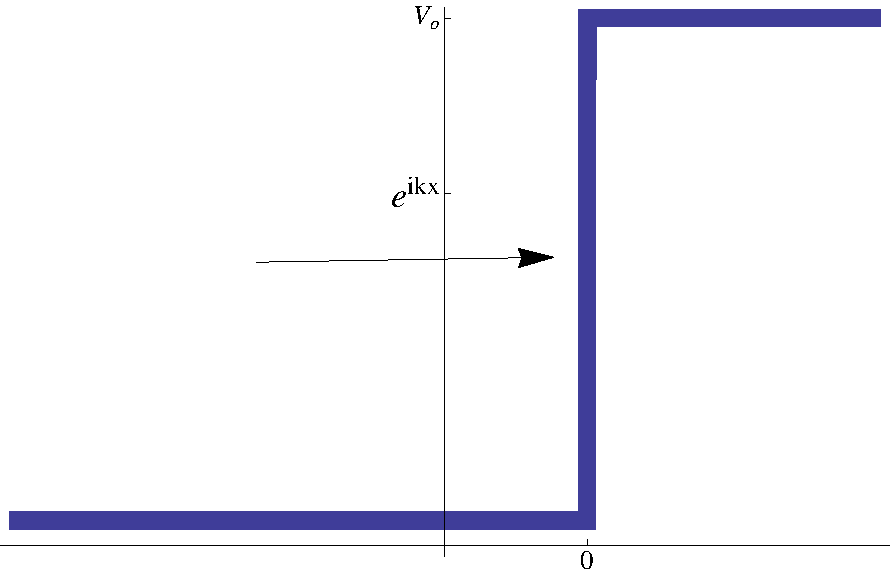
\includegraphics[scale=0.5]{barreira}
\end{center}


}

\frame{\frametitle{Barreira de Potencial}
  \begin{itemize}
  \item Discutir Importância
  \item Análogo Clássico
  \item Análogo Ótico
  \end{itemize}

}
\frame{\frametitle{Barreira de Potencial $E>V_o$}

$$-\frac{\hbar^2}{2m}\frac{d^2 u}{dx^2}+V(x)u(x)=Eu(x)$$

$$\frac{d^2 u}{dx^2}+\frac{2m}{\hbar^2}[E-V_o]u=0$$

$$k^2=\frac{2mE}{\hbar^2} \quad q^2=\frac{2m(E-V_o)}{\hbar^2}$$
}

\frame{\frametitle{Solução}

$$x<0$$

$$u(x)=e^{ikx}+Re^{-ikx}$$


$$j=\frac{\hbar}{2m}\left[ \psi^* \frac{\partial \psi}{\partial x}-
\psi \frac{\partial \psi^*}{\partial x}
\right]$$


$$j=\frac{\hbar k}{m}\left[1-|R|^2 \right]$$
}


\frame{\frametitle{Solução}
$$x>0$$

$$u(x)=Te^{iqx}$$

$$j=\frac{\hbar}{2m}q|T|^2$$

}

\frame{\frametitle{Condições sobre $u$}
Como determinar $R$  e $T$?

\begin{itemize}
\item $u$ é contínua.
\item a derivada de $u$ é contínua.
\end{itemize}
}


\frame{\frametitle{Derivada de $u$}

{\bf Teorema:} A derivada de $u$ é contínua em $x=0$.


\begin{eqnarray*}
\left(\frac{du}{dx} \right)_\epsilon-
\left(\frac{du}{dx} \right)_{-\epsilon}&=&
\int_{-\epsilon}^\epsilon dx \frac{d}{dx}\frac{du}{dx}\\
&=&
\int_{-\epsilon}^{\epsilon} dx \frac{2m}{\hbar^2}[V(x)-E]u(x)\\
&=&\int_{0}^{\epsilon} dx \frac{2m}{\hbar^2}[V_o-E]u(x)+
\int_{-\epsilon}^{0} dx \frac{2m}{\hbar^2}[-E]u(x) \\
&\sim& \frac{2m}{\hbar^2}\left\{ [V_o-E]u(-\epsilon) + Eu(\epsilon)\right\}\epsilon
\end{eqnarray*}

$$\lim_{\epsilon\rightarrow 0}\left(\frac{du}{dx} \right)_\epsilon-
\left(\frac{du}{dx} \right)_{-\epsilon}=0$$
}

\frame{\frametitle{Equações}
  \begin{equation*}
   u(x) =\left\{ 
\begin{array}{l l}
e^{ikx}+Re^{-ikx} & x<0 \\
Te^{iqx} & x\geq 0
\end{array}
\right.
  \end{equation*}

Em $x=0$ 
\begin{eqnarray*}
  \psi(0^+)&=&\psi(0^-)\\
u^\prime(0^+)&=&u^\prime (0^-)
\end{eqnarray*}
}



\frame{\frametitle{Equações}

  \begin{eqnarray*}
    1+R&=&T\\
k(1-R)&=&qT\\
  \end{eqnarray*}

$$R=\frac{k-q}{k+q} \quad T=\frac{2k}{k+q}$$
}

\frame{\frametitle{Equações}
Mostre que:

$$|R|^2+|T|^2=\frac{\hbar k}{m}$$

Qual é o significado físico disso?

}

\frame{\frametitle{Barreira de Potencial $E<V_o$}
  \begin{equation*}
   u(x) =\left\{ 
\begin{array}{l l}
e^{ikx}+Re^{-ikx} & x<0 \\
Te^{-|q|x} & x\geq 0
\end{array}
\right.
  \end{equation*}

Em $x=0$ 
\begin{eqnarray*}
 u(0^+)&=&u(0^-) \\
u^\prime(0^+)&=&u^\prime (0^-)
\end{eqnarray*}
}


\frame{\frametitle{Equações}

  \begin{eqnarray*}
    1+R&=&T\\
ik(1-R)&=&-|q|T\\
  \end{eqnarray*}

  $$R=\frac{ik+|q|}{ik-|q|} \quad T=\frac{2ik}{ik-|q|}$$

Note que:

$$\frac{\hbar k}{m}|R|^2=\frac{\hbar k}{m}$$

Ou seja todo fluxo incidente é refletido!
}


\section{Poço de Potencial}
\frame{\frametitle{Poço de Potencial}
\begin{center}
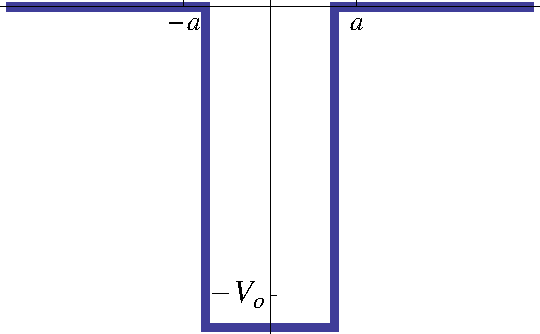
\includegraphics[scale=0.5]{poco}
\end{center}


}


\frame{\frametitle{Poço de Potencial $E>0$}
$$k^2=\frac{2mE}{\hbar^2} \quad q^2=\frac{2m(E+V_o)}{\hbar^2}$$
 \begin{equation*}
   u(x) =\left\{ 
\begin{array}{l l}
e^{ikx}+Re^{-ikx} & x<-a \\
Ae^{iqx}+Be^{-iqx} & -a<x<a \\
Te^{ikx} & x \geq a
\end{array}
\right.
  \end{equation*}
}

\frame{\frametitle{Equações}
  \begin{eqnarray*}
    1+R e^{-i a k}&=&A e^{-i a q}+B e^{i a q}\\
   -i k R e^{i ak}&=&i A q e^{-i a q}-i B q e^{i a
   q}\\ 
   A e^{i a q}+B e^{-i a q}&=&T
   e^{i a k}\\
   i A q e^{i a q}-i B q
   e^{-i a q}&=&i k T e^{i a   k}
  \end{eqnarray*}
}

\frame{\frametitle{Soluções}

Usando o Mathematica obtemos que 
$$T=$$
$$\frac{2 k q e^{i a (k+2 q)}}{k
   (k-q) \left(-e^{2 i a (k+2
   q)}\right)-q e^{4 i a q} (q-k)+k
   e^{2 i a k} (k+q)+q (k+q)}
$$
}
\frame{\frametitle{Barreira de Potencial}
\begin{center}
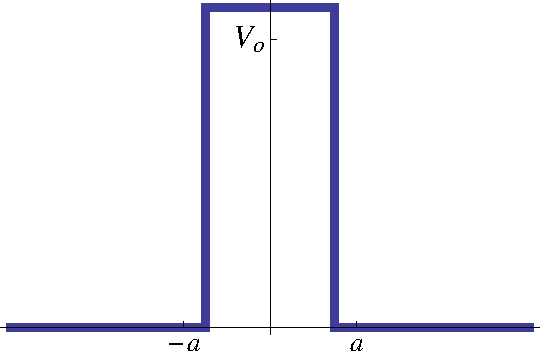
\includegraphics[scale=0.5]{barreira2}
\end{center}


}


\frame{\frametitle{Barreira de Potencial $E>0$}
$$k^2=\frac{2mE}{\hbar^2} \quad Q^2=\frac{-2m(E-V_o)}{\hbar^2}$$
 \begin{equation*}
   u(x) =\left\{ 
\begin{array}{l l}
e^{ikx}+Re^{-ikx} & x<-a \\
Ae^{-|Q|x}+Be^{|Q|x} & -a<x<a \\
Te^{ikx} & x \geq a
\end{array}
\right.
  \end{equation*}

Mesmo caso que o anterior se $q\rightarrow iQ$.
}

\frame{\frametitle{Soluções}

Usando o Mathematica obtemos uqe 
$$
T=\frac{4 k Q e^{2 a Q-2 i a k}}{i
   k^2 e^{4 a Q}-2 k Q e^{4 a Q}-i
   Q^2 e^{4 a Q}-i k^2-2 k Q+i Q^2}
$$

$$|T|^2=-\frac{8 k^2
   Q^2}{-\left(k^2+Q^2\right)^2
   \cosh (4 a Q)+k^4-6 k^2 Q^2+Q^4}$$
}


\frame{\frametitle{Transmitância}
\begin{center}
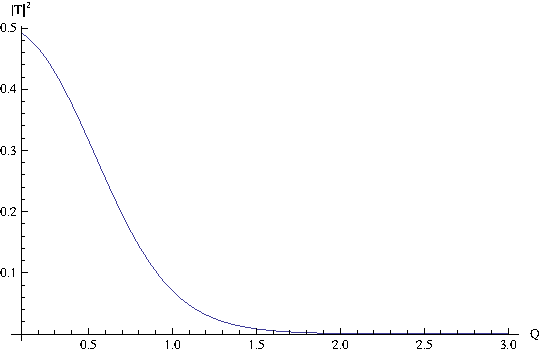
\includegraphics[scale=0.8]{transmi}
\end{center}
}

\frame{\frametitle{Aproximação WKB}
Quando $Qa>>1$ temos que:

$$|T|^2=\left( \frac{4 k Q}{k^2+Q^2}\right)e^{-4Qa}$$

$$\ln |T|^2\sim 2 \ln \left( \frac{4 k Q}{k^2+Q^2}\right) -(2Q)(2a)
\sim C -(2Q)(2a) \sim C-2Q\Delta$$ 

onde $\Delta$ é a largura do potencial.
}

\frame{\frametitle{Aproximação WKB}
WKB $\rightarrow$ Wentzel-Kramers-Brioullin
\begin{center}
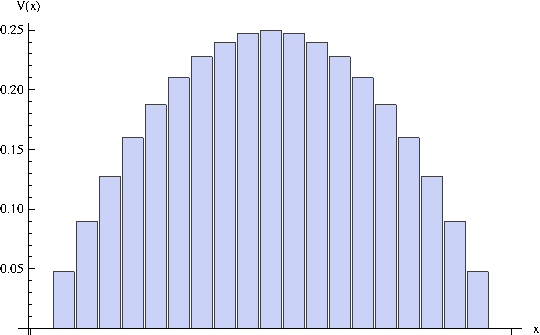
\includegraphics[scale=0.8]{wkb}
\end{center}
}


 \frame{\frametitle{Aproximação WKB}
 No caso de um potencial qualquer:

 $$|T|^2=|T_1|^2\ldots|T_N|^2$$

 $$\ln |T|^2\sim\sum_i \ln |T_i|^2\sim-2\sum_i \Delta_i Q_i$$

 $$=\sum_i \Delta_i \sqrt{2m (V(x_i)-E)/\hbar^2}$$ 

$$|T|^2=Ce^{-2 \int dx \sqrt{2m (V(x)-E)}}$$
 }

\frame{\frametitle{Aproximação WKB-Exemplo}
\begin{center}
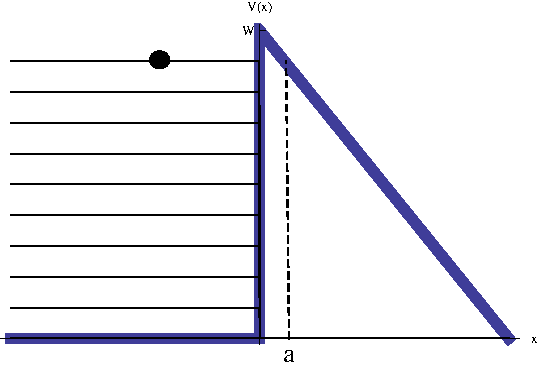
\includegraphics[scale=0.8]{eletron}
\end{center}
$$V(x)=W-e\epsilon x\quad a=\frac{W}{e\epsilon}$$
}
\frame{\frametitle{Aproximação WKB-Exemplo}
$$|T|^2=Ce^{-2 \int dx \sqrt{2m (V(x)-E)}}$$

$$|T|^2=C\exp \left[ -\frac{4\sqrt{2}}{3}\sqrt{\frac{Wma^2}{\hbar^2}}\right]$$
}


\frame{\frametitle{Poço de Potencial $E<0$}

$$\frac{2mE}{\hbar^2}=-\alpha^2\quad q^2=\frac{2m(V_o-|E|)}{\hbar^2}$$  
 \begin{equation*}
   u(x) =\left\{ 
\begin{array}{l l}
C_1e^{\alpha x} & x<-a \\
A \cos qx +B \sin qx & -a<x<a \\
C_2e^{-\alpha x} & x \geq a
\end{array}
\right.
  \end{equation*}
}


\frame{\frametitle{Equações}
  \begin{eqnarray*}
   C_1 e^{-a \alpha }&=&A
   \cos (a q)-B \sin (a q)\\
   A \cos
   (a q)+B \sin (a q)&=&C_2
   e^{-a \alpha }\\
  \alpha  C_1
   e^{-a \alpha }&=&A q \sin (a q)+B
   q \cos (a q)\\
  B q \cos (a q)-A q
   \sin (a q)&=&\alpha  -C_2
   e^{-a \alpha }
  \end{eqnarray*}
}


\frame{\frametitle{Soluções Caso Par}
Neste caso $B=0$.

\begin{eqnarray*}
C_1 e^{-a \alpha }&=&A
   \cos (a q)\\
A \cos (a
   q)&=&C_2e^{-a \alpha
   }\\
  \alpha  C_1 e^{-a \alpha
   }&=&A q \sin (a q)\\
  -A q \sin (a
   q)&=&\alpha  -C_2 e^{-a\alpha }
\end{eqnarray*}
}

\frame{\frametitle{Soluções Caso Par}
$$q\tan qa=\alpha$$

Definindo:

$$\lambda=\frac{2mV_oa^2}{\hbar^2}\quad y=qa$$

$$\tan y=\frac{\sqrt{\lambda -y^2}}{y}$$
}

\frame{\frametitle{Soluções Caso Par}
\begin{center}
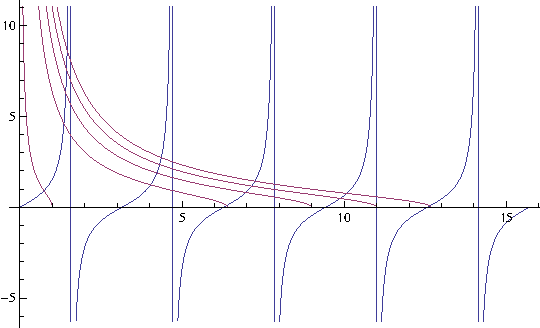
\includegraphics[scale=0.8]{poco3}
\end{center}
}

\frame{\frametitle{Equações Caso Impar}
Neste caso $A=0$.

\begin{eqnarray*}
C_1 e^{-a \alpha }&=&-B
   \sin (a q)\\
B \sin (a
   q)&=&C_2 e^{-a \alpha
   }\\
\alpha  C_1  e^{-a \alpha
   }&=&B q \cos (a q)\\
B q \cos (a
   q)&=&\alpha  -C_2 e^{-a
   \alpha }
\end{eqnarray*}
}

\frame{\frametitle{Soluções Caso Impar}
$$-\frac{1}{\tan y}=\frac{\sqrt{\lambda -y^2}}{y}$$

\begin{center}
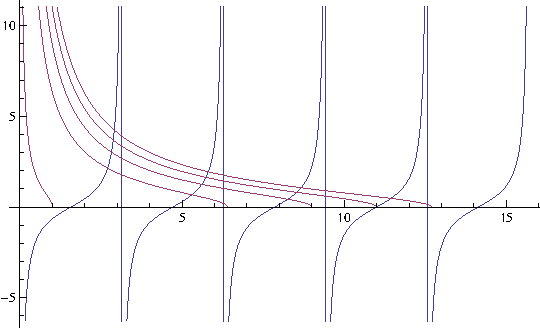
\includegraphics[scale=0.8]{poco4}
\end{center}
}

\frame{\frametitle{Resumo da Ópera}
  \begin{itemize}
  \item Dependendo de $\lambda$, ou seja da forma do poço
eu posso ter 1 ou mais estados ligados.
\item O número de estados ligados é sempre finito.
\item A cada estado corresponde um nível de energia, ou seja o espectro 
para esses sistemas é bastante complexo.
\item No limite em que $V_o$ tende a infinito recuperamos os níveis 
de energia para a partícula em uma caixa.
  \end{itemize}
}


\section{Oscilador Harmônico}
\frame{\frametitle{Hamiltoniano}
$$H=\frac{p^2}{2m}+\frac{kx^2}{2}$$

$$-\frac{\hbar^2}{2m}\frac{d^2u}{dx^2}+\frac{1}{2}kx^2u=Eu$$

$$\omega=\sqrt{\frac{k}{m}} \quad \epsilon=\frac{2E}{\hbar \omega}$$

$$y=\sqrt{\frac{m\omega}{\hbar}}x$$

}

\frame{\frametitle{Equação Diferencial}
$$
\frac{d^2 u}{dy^2}+(\epsilon-y^2)u=0
$$
}

\frame{\frametitle{Equação Diferencial Caso Limite}
Para $y>>0$

$$
\frac{d^2 u_o}{dx^2}-y^2u_o=0
$$

$$
\frac{du_o}{dy}\frac{d^2u_o}{dy^2}-y^2\frac{du_o}{dy}u_o=0
$$

$$
\frac{d}{dy}\left( \frac{du_o}{dy}\right)^2-y^2\frac{d(u_o)^2}{dy}=0
$$
}

\frame{\frametitle{Equação Diferencial Caso Limite}
$$
\frac{d}{dy}\left[ \left( \frac{du_o}{dy}\right)^2-y^2u_o^2\right]=-2yu_o^2\sim 0
$$

$$
 \left( \frac{du_o}{dy}\right)^2-y^2u_o^2=C
$$

$$
\frac{du_o}{dy}=\sqrt{C+y^2u_o^2}
$$
Quando $y\rightarrow\infty$ $u_o^2y^2\rightarrow 0$ temos:
}

\frame{\frametitle{Equação Diferencial Caso Limite}
$$\frac{du_o}{dy}\sim \sqrt{C}$$

Ou seja $C=0$.

$$\frac{du_o}{dy}=\pm yu_o$$

Só o caso negativo interessa:

$$u_o=Ae^{-y^2/2}$$.

$$
\frac{d}{dy}\left[ -4y^2e^{-y^2}-y^2e^{-y^2}\right]\sim y^3e^{-y^2}>>ye^{-y^2}
$$

}

\frame{\frametitle{Ans\"atz}
$$u(y)=h(y)e^{-y^2/2}$$
 Após algumas manipulações obtemos:

$$
h^{\prime\prime}-2yh^\prime+(\epsilon-1)h=0
$$
}

\frame{\frametitle{Comportamento Assintótico}

$$h(y)=\sum_{m=0}^\infty a_my^m$$

$$\sum_{m=0}^\infty\{(m+2)(m+1)a_{m+2}+[-2m+(\epsilon-1)]a_m\}$$

$$a_{m+2}=\frac{1-\epsilon+2 m}{(m+2)(m+1)}a_m$$

Obs. Os dois primeiros termos do primeiro termo desaparecem
}

\frame{\frametitle{Comportamento Assintótico}
$$a_{m+2}\sim\frac{a_m}{m/2}$$

$$
h(y)\sim a_o\left(1+y^2+\frac{y^4}{2!}+\ldots \right)=e^{y^2}
$$

$$u=h(y)e^{-y^2/2}\sim e^{y^2/2}$$

Ou seja $u$ diverge no infinito. Para evitar isso:
$$\epsilon=1+2n$$

$$\epsilon =\frac{2E}{\hbar \omega}$$
}

\frame{\frametitle{Polinômios de Hermite}

Reunindo estes resultados temos que:

$$E_n=\hbar \omega\left(n+\frac{1}{2} \right)$$

Além disso:

$$a_{m+2}=\frac{2(m-n)}{(m+1)(m+2)}a_m$$

Ou seja a série é truncada em $m=n$ e $h(y)$ se tornam 
polinômios, chamados de Polinômios de Hermite denotados por $H_n(y)$.

}

\frame{\frametitle{Polinômios de Hermite}

  \begin{eqnarray*}
    H_o(y)&=&a_o\\
    H_1(y)&=&ya_1\\
    H_2(y)&=&a_o\left(1-2 y^2 \right)
  \end{eqnarray*}
}

\frame{\frametitle{Autofunções}


$$u_m(y)=e^{-y^2/2}H(y)$$

$$\int_{-\infty}^\infty e^{-y^2}H_m(y)H_n(y) dy=\delta_{nm}$$

\begin{center}
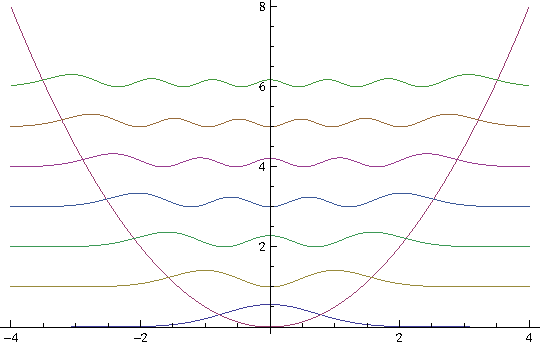
\includegraphics[scale=0.8]{hermite}
\end{center}

}



\frame{\frametitle{Exercício}
Considere partículas incidindo na direção positiva do eixo $x$ com $V_!<E<V_2$
e  escreva as equações que a função de onda deve obedecer. 


\begin{center}
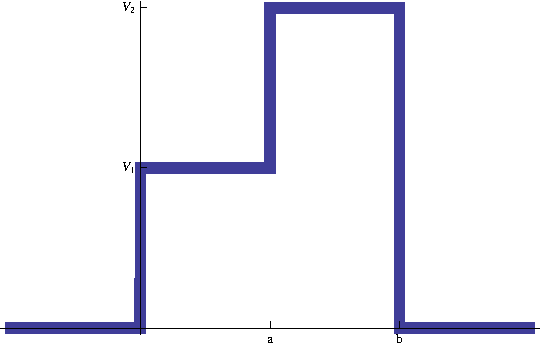
\includegraphics[scale=0.8]{potencialex}
\end{center}

}
\end{document}